\documentclass{beamer}

\mode<presentation> {
\usetheme{Madrid}
}

\usepackage{graphicx}
\usepackage{booktabs}
\usepackage[utf8]{inputenc} 
\usepackage[T1]{fontenc}
\usepackage[french]{babel}
\usepackage{listings}
%\usepackage{xcolor}
\usepackage{color}
\definecolor{bluekeywords}{rgb}{0.13,0.13,1}
\definecolor{greencomments}{rgb}{0,0.5,0}
\definecolor{redstrings}{rgb}{0.9,0,0}

\lstset{language=[Sharp]C,
  showspaces=false,
  showtabs=false,
  breaklines=true,
  showstringspaces=false,
  breakatwhitespace=true,
  escapeinside={(*@}{@*)},
  commentstyle=\color{greencomments},
  keywordstyle=\color{bluekeywords},
  stringstyle=\color{redstrings},
  basicstyle=\ttfamily
}

\usepackage{fontspec}
\usepackage{calc,lipsum}

\defbeamertemplate{section page}{mine}[1][]{%
  \begin{centering}
    {\usebeamerfont{section name}\usebeamercolor[fg]{section name}#1}
    \vskip1em\par
    \begin{beamercolorbox}[sep=12pt,center]{part title}
      \usebeamerfont{section title}\insertsection\par
    \end{beamercolorbox}
  \end{centering}
}

\defbeamertemplate{subsection page}{mine}[1][]{%
  \begin{centering}
    {\usebeamerfont{subsection name}\usebeamercolor[fg]{subsection name}#1}
    \vskip1em\par
    \begin{beamercolorbox}[sep=8pt,center,#1]{part title}
      \usebeamerfont{subsection title}\insertsubsection\par
    \end{beamercolorbox}
  \end{centering}
}

\setbeamertemplate{section page}[mine]
\setbeamertemplate{subsection page}[mine]

\AtBeginSection{\frame{\sectionpage}}
\AtBeginSubsection{\frame{\subsectionpage}}

\title[Introduction au C\#]{Introduction au C\#}

\author[]{
Nathan 'Njall' Gauër\\
Alexis 'Bmoc' Guiho\\
Quentin 'Neodyblue' Coelho
}
\institute[GConfs]
{
GConfs
\medskip
}
\date{13 Novembre 2015}

\begin{document}

\begin{frame}
\titlepage
\end{frame}

\begin{frame}
\frametitle{Déroulement}
\tableofcontents
\end{frame}

\section{Introduction}

\subsection{Présentation du langage}

\begin{frame}
\frametitle{Présentation}
\begin{itemize}
\item Inventé par Microsoft
\pause
\item Inspiré par Java, C++
\pause
\item Langage compilé
\pause
\item Fortement et statiquement typé
\pause
\item Impératif, orienté objet
\end{itemize}
\end{frame}

\begin{frame}
\frametitle{Compilation "classique"}
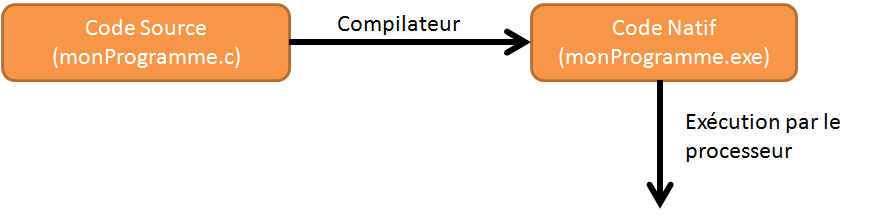
\includegraphics[scale=0.50]{img/comp_nat.png}
\end{frame}

\begin{frame}
\frametitle{Compilation en C\#}
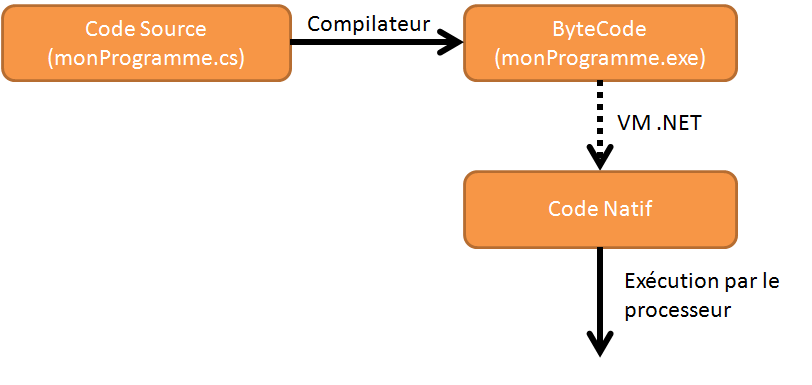
\includegraphics[scale=0.40]{img/comp_bc.png}
\end{frame}

\subsection{.NET}

\begin{frame}
\begin{itemize}
\frametitle{.NET}
\item Framework développé par Microsoft
\item Bibliothèque de classes
\item Utilisable via plusieurs langages (C\#, VB .Net, F\#, J\# ...)
\item Common Language Infrastructure
\end{itemize}
\end{frame}

\begin{frame}
\begin{center}
\frametitle{.NET CLI}
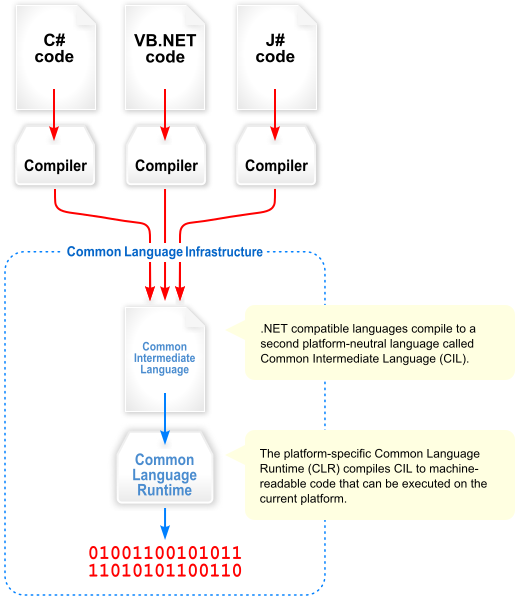
\includegraphics[scale=0.38]{img/cli.png}
\end{center}
\end{frame}

\section{Syntaxe}
\subsection{Types basiques}

\begin{frame}[fragile]
\frametitle{Déclaration d'une variable}
\begin{center}
\begin{lstlisting}
<type> <nom>;
<type> <nom> = <valeur>;
\end{lstlisting}
\pause
\begin{lstlisting}
<type>[] <nom>;
<type>[] <nom> = <variable>;
<type>[] <nom> = new <type>[<taille>];
\end{lstlisting}
\end{center}
\end{frame}

\begin{frame}[fragile]
\frametitle{Cas pratiques}
\begin{center}
\begin{lstlisting}
int toto = 42;
int tata = toto;
float answer = 4.2;
double mille = 1000.0;
long beaucoup = 27972000000000;
bool faux = false;
bool vrai = true;
string votay = "Test.";
int[] jesuisuntableau = new int[100];
int[] jesuislememetableau = jesuisuntableau;
\end{lstlisting}
\end{center}
\end{frame}

\begin{frame}[fragile]
\frametitle{Opérations basiques}
\begin{columns}[T]

\begin{column}{.48\textwidth}
Opérateurs classiques
\begin{itemize}
\item +(=)
\item -(=)
\item *(=)
\item /(=)
\item \%(=)
\end{itemize}
\end{column}

\hfill

\begin{column}{.48\textwidth}
Opérateurs de comparaison
\begin{itemize}
\item ==
\item !=
\item \textless (=)
\item \textgreater (=)
\end{itemize}
\end{column}

\end{columns}
\end{frame}

\begin{frame}[fragile]
\frametitle{Par l'exemple}
\begin{center}
\begin{lstlisting}
int answer = 20 * 2 + 2;
//answer <- 42
answer += 2
//answer <- 44
bool vrai = answer == 44;
//vrai <- true
bool faux = (answer % 2) == 1;
//faux <- false
string question = "Quelle est la " + "question ?";
// question <- Quelle est la question ?
\end{lstlisting}
\end{center}
\end{frame}

\begin{frame}[fragile]
\frametitle{Utilisation des tableaux}
\begin{center}
\begin{lstlisting}
int[] toto = new int[2];
toto[0] = 42;
//On assigne 42 dans la case zero
toto[1] = -21;
//On assigne -21 dans la case une
toto[2] = 0;
//On crash lamentablement...
\end{lstlisting}
\end{center}
\end{frame}

\begin{frame}[fragile]
\frametitle{Warning}
\begin{lstlisting}
int foo = 42;
int bar = foo;
bar = 21;
\end{lstlisting}
Que vaut foo ?
\pause
Réponse: 42
\pause
\begin{lstlisting}
int[] foo = new int[2];
foo[0] = 42;
int[] bar = foo;
bar[0] = 21;
\end{lstlisting}
Que vaut foo[0] ?
\pause
Réponse: 21
\end{frame}

\begin{frame}[fragile]
\frametitle{Déclaration de fonction}
\begin{lstlisting}
<type> <nom>(<type1> <param1>, <type2> <param2>)
{
    //Corps de la fonction
    //...
    return <value of type <type>>;
}
\end{lstlisting}
\pause
\begin{lstlisting}
int mult(int a)
{
    return a * 2;
}

void do_something(int a, int b)
{
    //do not need a return
}
\end{lstlisting}
\end{frame}

\begin{frame}[fragile]
\frametitle{Appel de fonction}
\begin{lstlisting}
int test = mult(500);
int test_2 = mult(test);
do_something(test, test_2);
\end{lstlisting}
\end{frame}

\subsection{Programmation impérative}

\begin{frame}[fragile]
\frametitle{Mon ordinateur, mon esclave}
\begin{itemize}
\item<+-> Fais moi un sandwhich;
\item<+-> Fais la vaisselle;
\item<+-> Sors les poubelles;
\item<+-> Répare la plomberie
\item<+-> Tant que (le sol est sale):\\
	\{ Lave le sol; \}
\item<+-> Si (il y a du courrier):\\
	\{ Va chercher le courrier; \}
\end{itemize}
\pause
Il obéit.
\end{frame}

\begin{frame}[fragile]
\frametitle{Structure de contrôle - if}
\begin{lstlisting}
if (<condition>) {
    <instructions>
} else if (<condition>) { //Optionnel
    <instructions>
} else if (<condition>) { //Optionnel
    <instructions>
} else { //Optionnel
    <instructions>
}
\end{lstlisting}
\end{frame}

\begin{frame}[fragile]
\frametitle{Par l'exemple}
\begin{lstlisting}
int year = 2020;
if (year % 2 == 1) {
    Console.Writeline("Une promo qui respire la qualitay");
} else if (year == 2020) {
    Console.Writeline("Tout n'est pas perdu !");
} else {
    Console.Writeline("Il va falloir s'accrocher...");
}
\end{lstlisting}
\end{frame}

\begin{frame}[fragile]
\frametitle{Structure de contrôle - switch}
\begin{lstlisting}
switch (<variable>){
    case <cas 1>:
        <instructions>
        break;
    case <cas 2>:
        <instructions>
        break;
    default:
        <instructions>
        break;
}
\end{lstlisting}
\end{frame}

\begin{frame}[fragile]
\frametitle{Par l'exemple}
\begin{lstlisting}
int year = 2020;
switch(year){
    case 2000:
        Console.Writeline("Buggy prom..");
        break;
    case 2020:
        Console.Writeline("Tout n'est pas perdu !");
        break;
    default:
        Console.Writeline("On s'accroche !");
        break;
}
\end{lstlisting}
\end{frame}

\begin{frame}[fragile]
\frametitle{Structure de contrôle - while - do while}
\begin{lstlisting}
while(<condition>) {
    <instructions>
}

do {
    <instructions>
} while(<condition>);
\end{lstlisting}
\end{frame}

\begin{frame}[fragile]
\frametitle{Par l'exemple}
\begin{lstlisting}
int i = 1;
while (i < 42)
{
    i = i * 2;
}
\end{lstlisting}
\begin{lstlisting}
string name = "";
do {
    Console.WriteLine("Entrez votre nom");
    name = Console.ReadLine();
} while (name == "");
\end{lstlisting}
\end{frame}

\begin{frame}[fragile]
\frametitle{Structure de contrôle - for}
\begin{lstlisting}
for (<initial>; <condition>; <instructions>) {
    <instructions>
}
\end{lstlisting}
\end{frame}

\begin{frame}[fragile]
\frametitle{Par l'exemple}
\begin{lstlisting}
int[] array = new int[10];
array[0] = 1;
for (int i = 1; i < array.Length; ++i) {
    array[i] = i * array[i - 1];
}

for (int i = 0; i < array.Length; ++i) {
    Console.WriteLine(array[i]);
}
// 1, 1, 2, 6, 24...
\end{lstlisting}
\end{frame}

\section{Programmation orientée objet}

\subsection{Présentation}

\begin{frame}
\frametitle{La POO ?}
\begin{itemize}
\item Paradigme
\item Entités appelées "objets"
\item Structure des objets définie par les "classes"
\end{itemize}
\end{frame}

\begin{frame}
\frametitle{Un objet}
\begin{itemize}
\item Des valeurs: "champs"
\item Des fonctions appartenant à l'objet: "methodes"
\end{itemize}
\end{frame}

\begin{frame}[fragile]
\frametitle{Une classe}
La classe est à l'objet ce que le moule est au gateau.\\
Décrit la structure et la composition d'un objet: c'est un plan de conception.
\begin{lstlisting}
class Test
{
    // contenu de la classe: champs, methodes
}
\end{lstlisting}
\end{frame}

\begin{frame}
\frametitle{Une classe}
\begin{itemize}
\item Une classe A : "Plan" décrivant des méthodes et des champs.
\item Une instance de A : Objet utilisable, ayant la forme et la structure définies par A.
\end{itemize}
\end{frame}

\begin{frame}[fragile]
\frametitle{Les champs}
Les champs d'une classe sont définis comme des variables.
\begin{lstlisting}
class Voiture
{
    //Champs
    int vitesse;
    bool passager_bavard;
    string carburant;
}
\end{lstlisting}
\end{frame}

\begin{frame}[fragile]
\frametitle{Une classe}
Les methodes sont des fonctions définies à l'intérieur de la classe, permettant d'intéragir avec l'objet.
\begin{lstlisting}
class Voiture
{
    //Champs
    [...]
    //Methodes
    void accelerer();
    void klaxonner();
    void ejecter_passager();
}
\end{lstlisting}
\end{frame}

\begin{frame}[fragile]
\frametitle{Une classe}
Pour utiliser cette voiture, il faut en construire une ...
\end{frame}

%\begin{frame}[fragile]
%\frametitle{Une classe}
%Une fois construite, on peut l'utiliser.
%\begin{lstlisting}
%Voiture v = new Voiture();
%v.accelerer();
%\end{lstlisting}
%\end{frame}

%\begin{frame}[fragile]
%\frametitle{Une classe}
%Mais les attributs dans tout ça ?\\
%\end{frame}

%\begin{frame}[fragile]
%\frametitle{Une classe}
%Mais les attributs dans tout ça ?\\
%La classe est un plan; On nous dit :
%\begin{quotation}
%\lowbiglquote
%Dans les voitures que tu construira, un int vitesse tu mettra.
%\lowbigrquote\\
%-Yoda
%\end{quotation}
%\end{frame}

%\begin{frame}[fragile]
%\frametitle{Une classe}
%Ainsi chaque object fabriqué (on parle de classe instanciée) dispose de ses propres attributs.
%\begin{lstlisting}
%Voiture A = new Voiture();
%Voiture B = new Voiture();

%A.passager_bavard = true;
%B.passager_bavard = false;

%if(A.passager_bavard)
%    A.ejecter_passager();
%if(B.passager_bavard)
%    B.ejecter_passager();

%\end{lstlisting}
%\end{frame}

\subsection{Créer et manipuler des objets}

\begin{frame}[fragile]
\frametitle{Création d'un objet}
Aussi appellé "instanciation" car il s'agit de créer une instance d'une classe.
\begin{lstlisting}
<type> var = new <type>();
\end{lstlisting}
\end{frame}

\begin{frame}[fragile]
\frametitle{Une methode particulière: le constructeur}
Il est appellé lorsque l'objet est créé, permet d'effectuer des actions lors de la création.
\begin{lstlisting}
class Point
{
    int x;
    int y;
    
    public Point() {
        Console.WriteLine("On est à l'interieur du constructeur");
    }
}
...
Point p = new Point(); // Affiche un message sur la console
\end{lstlisting}
\end{frame}

\begin{frame}[fragile]
\frametitle{Une methode particulière: le constructeur}
Il peut prendre des paramètres, comme une fonction.
\begin{lstlisting}
class Point
{
    int x;
    int y;

    public Point(int x, int pos_y) {
        this.x = x;
        y = pos_y;
    }
}
// Créer un Point dont les champs x et y vaudront 3 et 5
Point p1 = new Point(3, 5);
// Un second, dont les champs x et y vaudront 4 et 2
Point p2 = new Point(4, 2);
\end{lstlisting}
\end{frame}

\begin{frame}
\frametitle{Une methode particulière: le constructeur}
\begin{alertblock}{Constructeur par défaut}
Un constructeur vide ne prenant aucun paramètre est utilisé par défaut si aucun constructeur n'a été défini.
\end{alertblock}
\end{frame}

\subsection{La visibilité}

\begin{frame}[fragile]
\frametitle{La visibilité}
La visibilité permet de définir les éléments de l'objet qui seront accessibles par ceux qui manipuleront cet objet.\\
La visibilité est intégrée la définition des éléments dans la classe.\\
\begin{lstlisting}
class Test
{
    <visibilité> <élément>
}
\end{lstlisting}
\end{frame}

\begin{frame}
\frametitle{La visibilité}
Il existe plusieurs types de visibilité, voici les plus simples:
\begin{itemize}
\item public: accessible de l'intérieur de l'objet et de l'exterieur
\item private: accessible uniquement de l'intérieur de l'objet
\end{itemize}
\begin{alertblock}{Visibilité par défaut}
Si la visibilité n'est pas définie, elle est private par défaut.
\end{alertblock}
\end{frame}

\begin{frame}[fragile]
\frametitle{Exemples de visibilité}
\begin{lstlisting}
class Test
{
    public int a;
    string b;
    private int c;
}

Test obj = new Test();
int val1 = obj.a; // OK
string val2 = obj.b; // Erreur, b private
int val3 = obj.c; // Erreur, c private
\end{lstlisting}

\end{frame}

\begin{frame}[fragile]
\frametitle{Exemples de visibilité}
\begin{lstlisting}
class CreditCard
{
    private int code = 4321;
    
    public void Pay(int given_code, float price)
    {
        if (given_code == this.code)
        {
            // Pay
        }
    }
}
\end{lstlisting}
\end{frame}

\subsection{Utilisation}

\begin{frame}[fragile]
\frametitle{Revenons à notre point}
\begin{lstlisting}
class Point
{
    int x;
    int y;

    public Point(int x, int pos_y) {
        this.x = x;
        y = pos_y;
    }
}
Point p = new Point(3, 4);
Console.WriteLine(p.x); // Erreur
\end{lstlisting}
\begin{alertblock}{Erreur de visibilité}
Les champs x et y ne sont pas accessibles.
\end{alertblock}
\end{frame}

\begin{frame}[fragile]
\frametitle{Revenons à notre point}
\begin{lstlisting}
class Point
{
    public int x;
    public int y;
    
    public Point(int x, int pos_y) {
        this.x = x;
        y = pos_y;
    }
}
Point p = new Point(3, 4);
Console.WriteLine(p.x); // Affiche 3
\end{lstlisting}
\end{frame}

\begin{frame}[fragile]
\frametitle{Une dernière chose ...}
\begin{lstlisting}
Point p = new Point(4,2);
Point aux = p;
aux.x = 2;
\end{lstlisting}
Question: que vaut p.x ? 
\pause
Réponse: 2
\end{frame}

\subsection{Héritage}
\begin{frame}
\frametitle{Un premier pas dans le monde de l'héritage}
Une classe (fille) peut hériter d'une autre classe (mère), cela signifie que
\begin{itemize}
\item La classe fille à accès aux champs et méthodes "protected" de la classe mère.
\item Une instance fille peut être vue comme une instance mère
\item Une instance fille peut redéfinir certaines méthodes de la classe mère
\end{itemize}
\pause
Cela permet de factoriser du code\\
\pause
La relation mère-fille peut se définir comme: la fille est une mère.
\end{frame}

\begin{frame}[fragile]
\frametitle{Un héritage classique}
\begin{lstlisting}
class Animal {
    string nom;
    public Animal(string nom) {
        this.nom = nom;
    }
}
class Chat : Animal {
    public Chat(string nom) : base(nom) {
    }
}

Animal noisette = new Chat("Noisette");
Animal[] ferme = new Animal[10];
ferme[0] = noisette;
ferme[1] = new Vache("Lucette");
ferme[2] = new Canard("Saturnin");
\end{lstlisting}
\end{frame}

\begin{frame}[fragile]
\frametitle{Méthode standard}
\begin{lstlisting}
class Animal {
    public string GetNom() { return nom; }
}
class Chat : Animal {
    public void Miaule() {Console.WriteLine("Miaou");}
}

Chat noisette = new Chat("noisette");
noisette.Miaule(); //OK
noisette.GetNom(); //OK
Animal noisette_bis = noisette;
noisette_bis.GetNom(); //OK
noisette_bis.Miaule(); //KO
\end{lstlisting}
\end{frame}


\begin{frame}[fragile]
\frametitle{Méthode virtuelle}
\begin{lstlisting}
class Animal {
    virtual void Shout() {
        Console.Writeline("...");
    }
}
class Chat : Animal {
     override void Shout() {
         Console.Writeline("Miaou !");
     }
}
bob = new Animal("bob");
bob.Shout(); //...
bob = new Chat("noisette");
bob.Shout(); //Miaou
\end{lstlisting}
\end{frame}

\subsection{Namespaces}

\begin{frame}
\frametitle{Première approche}
\begin{itemize}
\item Les namespaces sont des "boites" dans lesquelles on trouve un ensemble de classes ayant une relation entre elles (calcul, gestion du réseau, des fichiers...).
\item Les namespaces peuvent s'imbriquer.
\item Il existe une visibilité entre les namespaces, ainsi on peut déclarer une classe publique (elle peut être vue à l'exterieur du namespace) ou privée (elle n'est vue qu'a l'interieur).

\end{itemize}
\end{frame}

\begin{frame}[fragile]
\frametitle{Utiliser un namespace}
Pour accéder à une classe présente dans un namespace, deux choix s'offrent à nous.
\begin{lstlisting}
System.IO.FileInfo file = 
    new System.IO.FileInfo("pown.pdf");
\end{lstlisting}
\pause
\begin{lstlisting}
using System.IO;

//...

FileInfo file = new FileInfo("pown.pdf");
\end{lstlisting}
\end{frame}

\begin{frame}[fragile]
\frametitle{Mon namespace à moi}
\begin{lstlisting}
namespace Toto
{
    // code
}
\end{lstlisting}
\pause
\begin{lstlisting}
namespace Toto
{
    namespace Tata
    {
        // code
    }
}
\end{lstlisting}
\end{frame}

\section{Questions ?}

\end{document}
